\begin{block}{Partitions interactives}
\begin{figure}
    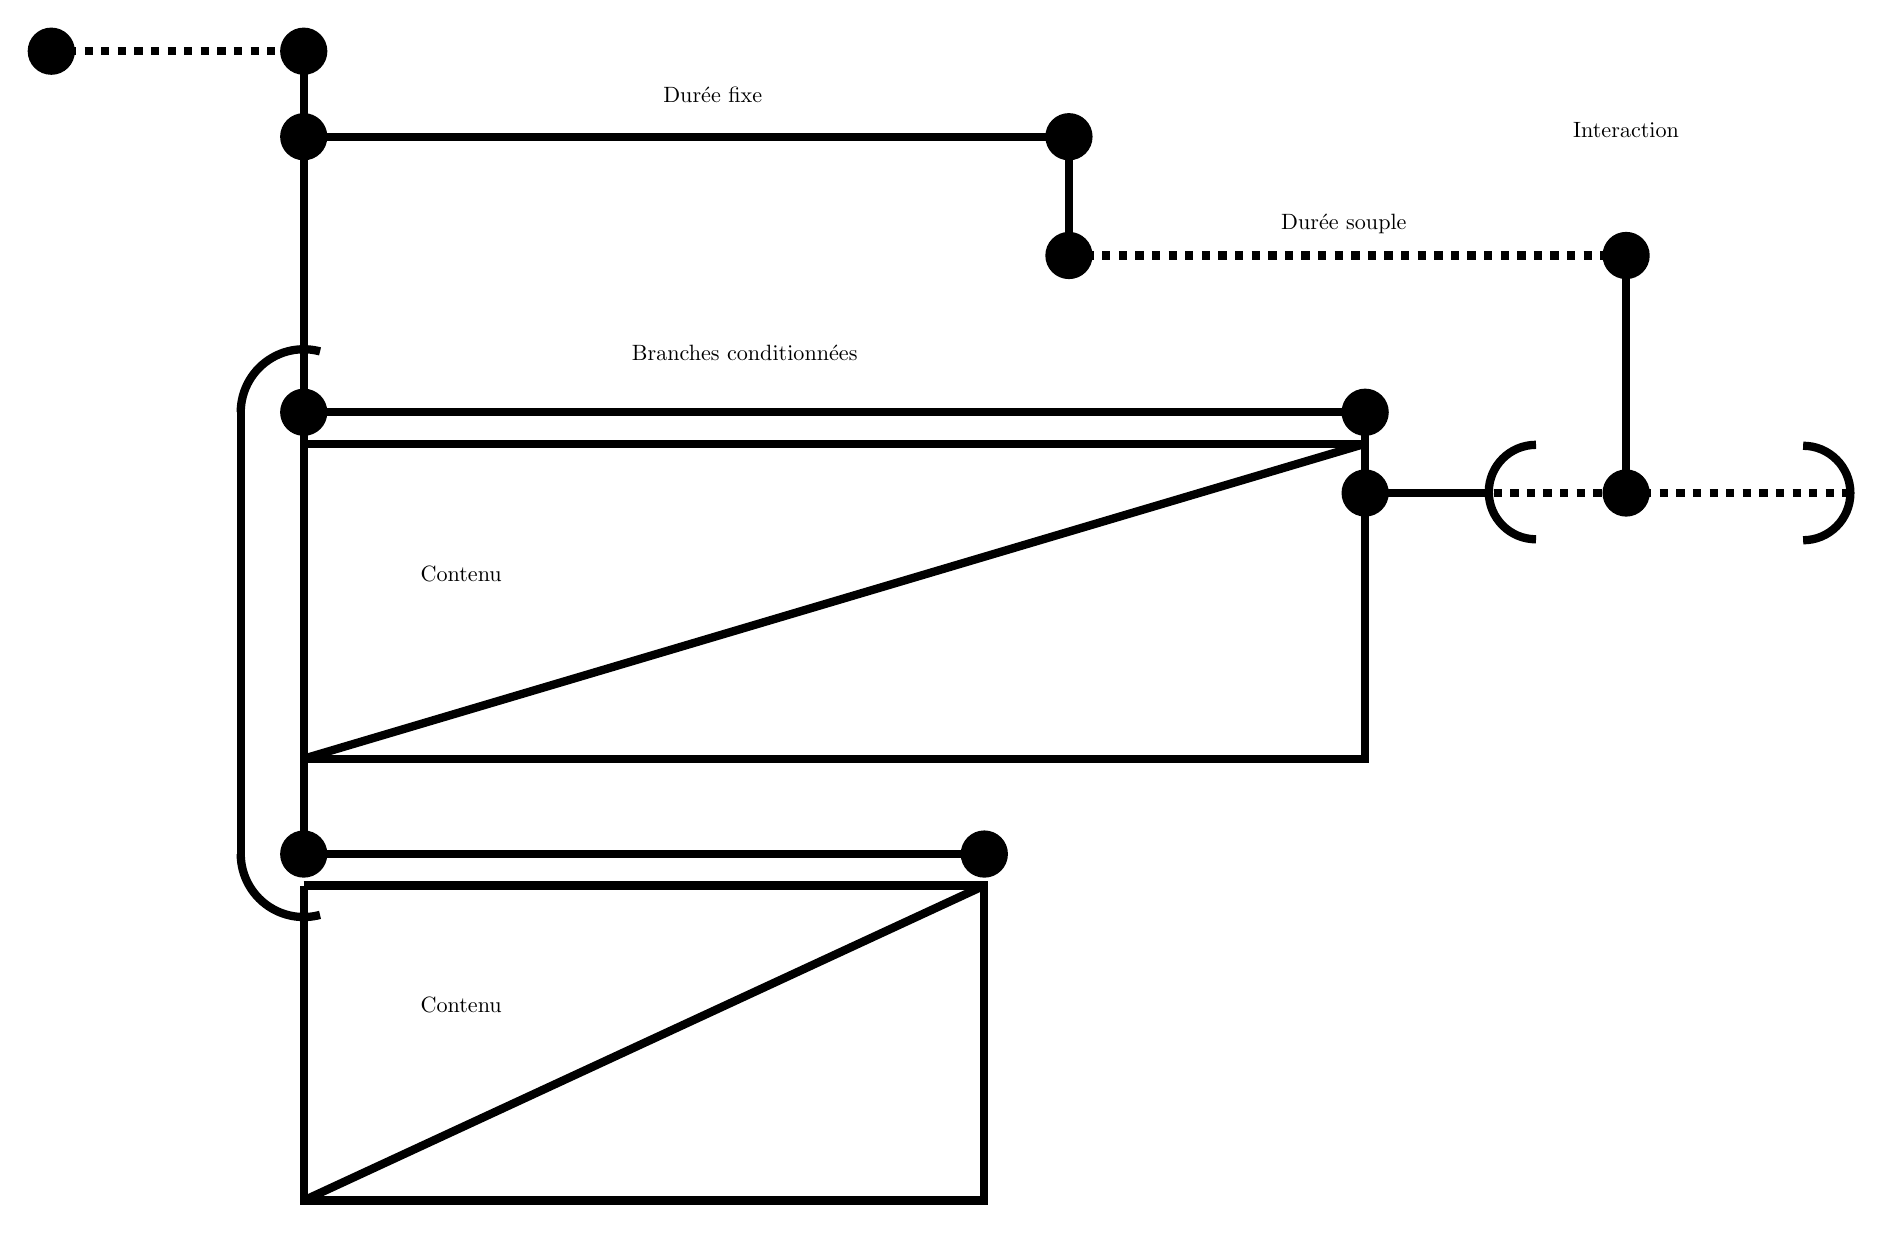
\begin{tikzpicture}[scale=4, every node/.style={scale=0.8}]
\fill (0, 21.6585) circle (0.075) ; % State.1 
\fill (0.801509, 21.6585) circle (0.075) ; % State.2 
\fill (0.801509, 20.5122) circle (0.075) ; % State.3 
\fill (4.1715, 20.5122) circle (0.075) ; % State.4 
\fill (0.801509, 21.387) circle (0.075) ; % State.5 
\fill (3.23104, 21.387) circle (0.075) ; % State.6 
\fill (3.23104, 21.0099) circle (0.075) ; % State.7 
\fill (5, 21.0099) circle (0.075) ; % State.8 
\fill (4.1715, 20.2558) circle (0.075) ; % State.9 
\fill (5, 20.2558) circle (0.075) ; % State.10 
\fill (0.801509, 19.1095) circle (0.075) ; % State.11 
\fill (2.96233, 19.1095) circle (0.075) ; % State.12 
\draw[line width=3pt] (0, 21.6585)  -- (0, 21.6585) ; % TimeNode.0 
\draw[line width=3pt] (0.801509, 21.6585)  -- (0.801509, 19.1095) ; % mule87fens83 
\draw[line width=3pt] (4.1715, 20.5122)  -- (4.1715, 20.2558) ; % zero63aunt55 
\draw[line width=3pt] (3.23104, 21.387)  -- (3.23104, 21.0099) ; % dell37didn59 
\draw[line width=3pt] (5, 21.0099)  -- (5, 20.2558) ; % brow57jill79 
\draw[line width=3pt] (2.96233, 19.1095)  -- (2.96233, 19.1095) ; % many97grid9 
\draw[dashed,line width=3pt] (0, 21.6585)  -- (0.801509, 21.6585) ; % slog45felt83 
\draw[line width=3pt] (0.801509, 20.5122)  -- (4.1715, 20.5122) ; % volume 
\draw[line width=3pt] (0.801509, 20.4122)  -- (4.1715, 20.4122)  -- (4.1715, 19.4122)  -- (0.801509, 19.4122)  -- (0.801509, 20.4122) ;
\draw[line width=3pt] (0.801509, 19.4122)  -- (4.1715, 20.4122) ;
\draw[line width=3pt] (0.801509, 21.387)  -- (3.23104, 21.387) ; % ears55auto57 
\draw[dashed,line width=3pt] (3.23104, 21.0099)  -- (5, 21.0099) ; % cole68beet23 
\draw[line width=3pt] (4.1715, 20.2558)  -- (4.574, 20.2558) ; % nate5just59 
\draw[dashed,line width=3pt] (4.474, 20.2558)  -- (5.71206, 20.2558) ; % nate5just59 
\draw[line width=3pt] (4.714, 20.4088) arc(90:270:0.15) ; % nate5just59 
\draw[line width=3pt] (5.56206, 20.1058) arc(-90:90:0.15) ; % nate5just59 
\draw[line width=3pt] (0.801509, 19.1095)  -- (2.96233, 19.1095) ; % lumiere 
\draw[line width=3pt] (0.801509, 19.0095)  -- (2.96233, 19.0095)  -- (2.96233, 18.0095)  -- (0.801509, 18.0095)  -- (0.801509, 19.0095) ;
\draw[line width=3pt] (0.801509, 18.0095)  -- (2.96233, 19.0095) ;
\draw[line width=3pt] (0.601509, 20.5122)  -- (0.601509, 19.1095) ; % adds31aloe19 
\draw[line width=3pt] (0.601509, 20.5122) arc(180:75:0.2) ; % adds31aloe19 
\draw[line width=3pt] (0.601509, 19.1095) arc(180:285:0.2) ; % adds31aloe19 


\draw (2.1, 21.5199) node {Durée fixe};
\draw (4.104, 21.1099) node {Durée souple};
\draw (2.201509, 20.7) node {Branches conditionnées};
\draw (1.301509, 20) node {Contenu};
\draw (1.301509, 18.6295) node {Contenu};
\draw (5, 21.4099) node {Interaction};
\end{tikzpicture}
\caption{Syntaxe d'une partition interactive}
\end{figure}
Possibilités d'écritures forment un langage de programmation structuré axé sur l'organisation temporelle. 
\textbf{Boucles} et \textbf{hiérarchie}, calcul instantané ou temporel possible via \textbf{Javascript}.
Applications : musique interactive, scénographie et spectacle vivant, contrôle de robots.

Répartition bas-niveau fait déjà partie du formalisme : envoi de messages entre applications, synchronisation, etc.
\end{block}
\begin{block}{Applications visées}
    \begin{itemize}
        \item \textbf{Murs d'écrans} vidéo.
        \item Installations artistiques polyphoniques et ouvertes~: 
        par exemple permettre d'utiliser la présence de \textbf{plusieurs appareils mobiles} 
        lors de l'écriture.
        \item \textbf{Back-up} à chaud des régies de spectacle.
        \item Réduction de gigue sur périphériques embarqué.
    \end{itemize}
\end{block}